\documentclass[11pt]{article}
\usepackage[a4paper, margin=1in]{geometry}
\usepackage{amsmath}
\usepackage{graphicx}
\usepackage{tikz}
\usepackage{amsfonts}
\usepackage{amssymb}

\title{\textbf{Lesson Plan: Mastering Standing Waves (1 Hour)}}
\author{}
\date{}

\begin{document}

\maketitle

Our goal today is to understand the physics of standing waves on a string and apply it to solve these four challenging problems. We'll break it down into three parts:
\begin{enumerate}
    \item \textbf{The Core Physics \& Equations:} The essential tools you need.
    \item \textbf{Advanced Concepts:} Buoyancy, beats, and alloys.
    \item \textbf{Problem-Solving Strategy:} How to attack each problem.
\end{enumerate}

\hrulefill

\section{Part 1: The Core Physics \& Equations (15 mins)}

The behavior of a wave on a string, like a guitar string, is governed by a few key relationships.

\subsection{Wave Speed on a String ($v$)}

The speed of a transverse wave traveling along a stretched string depends on two things: how tight the string is (\textbf{tension}) and how heavy it is (\textbf{linear mass density}).

The equation is:
$$v = \sqrt{\frac{F_T}{\mu}}$$

\begin{itemize}
    \item $F_T$ is the \textbf{tension} in the string (in Newtons, N). This is the force stretching the string. In many problems, this is provided by a hanging mass, so $F_T = mg$.
    \item $\mu$ is the \textbf{linear mass density}, which is the mass per unit length of the string (in kg/m).
\end{itemize}

\textbf{Crucially}, there are two ways to find $\mu$:
\begin{enumerate}
    \item If you know the total mass ($m_{wire}$) and total length ($L_{wire}$): $\mu = \frac{m_{wire}}{L_{wire}}$
    \item If you know the material's density ($\rho$) and cross-sectional area ($A$): $\mu = \rho \times A$. For a circular wire with diameter $D$ or radius $r$, the area is $A = \pi r^2 = \frac{\pi D^2}{4}$.
\end{enumerate}

\subsection{Standing Waves: Harmonics \& Frequency}

When a string is fixed at both ends (length $L$), it can only vibrate at specific resonant frequencies, creating patterns called \textbf{standing waves}. These are called \textbf{harmonics}.

\begin{center}
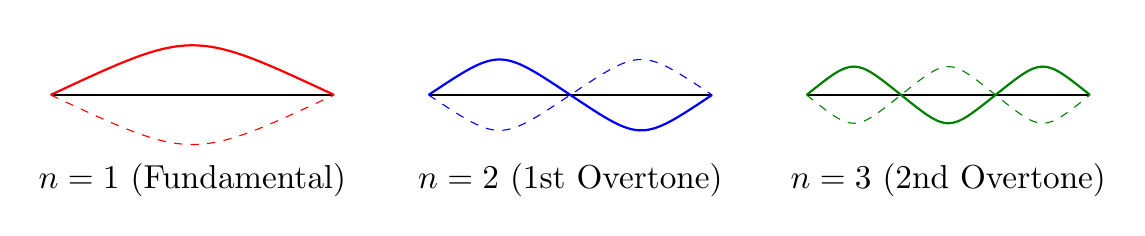
\begin{tikzpicture}[scale=1.2, every node/.style={transform shape}]
    % n=1
    \draw[thick] (0,0) -- (3,0);
    \draw[thick, red] (0,0) .. controls (1.5,0.7) and (1.5,0.7) .. (3,0);
    \draw[dashed, red] (0,0) .. controls (1.5,-0.7) and (1.5,-0.7) .. (3,0);
    \node at (1.5, -0.9) {$n=1$ (Fundamental)};
    
    % n=2
    \draw[thick] (4,0) -- (7,0);
    \draw[thick, blue] (4,0) .. controls (4.75,0.5) and (4.75,0.5) .. (5.5,0) .. controls (6.25,-0.5) and (6.25,-0.5) .. (7,0);
    \draw[dashed, blue] (4,0) .. controls (4.75,-0.5) and (4.75,-0.5) .. (5.5,0) .. controls (6.25,0.5) and (6.25,0.5) .. (7,0);
    \node at (5.5, -0.9) {$n=2$ (1st Overtone)};
    
    % n=3
    \draw[thick] (8,0) -- (11,0);
    \draw[thick, green!50!black] (8,0) .. controls (8.5,0.4) .. (9,0) .. controls (9.5,-0.4) .. (10,0) .. controls (10.5,0.4) .. (11,0);
    \draw[dashed, green!50!black] (8,0) .. controls (8.5,-0.4) .. (9,0) .. controls (9.5,0.4) .. (10,0) .. controls (10.5,-0.4) .. (11,0);
    \node at (9.5, -0.9) {$n=3$ (2nd Overtone)};
\end{tikzpicture}
\end{center}

The frequency of the n-th harmonic ($f_n$) is given by:
$$f_n = n \left( \frac{v}{2L} \right) \quad \text{for } n = 1, 2, 3, \ldots$$

\begin{itemize}
    \item $L$ is the vibrating length of the string (e.g., the distance between the bridges on a sonometer).
    \item $n$ is an integer called the \textbf{harmonic number}. It represents the number of "loops" or antinodes you see on the string.
    \item \textbf{Fundamental Frequency ($n=1$):} This is the lowest possible frequency.
    \item \textbf{Overtones:} These are the harmonics above the fundamental. The \textbf{first overtone} is the second harmonic ($n=2$), the \textbf{second overtone} is the third harmonic ($n=3$), and so on.
\end{itemize}

\subsection{The "Master Equation"}

By substituting the equation for wave speed into the frequency equation, we get the single most important formula for these problems:

$$f_n = \frac{n}{2L} \sqrt{\frac{F_T}{\mu}}$$

Almost every problem starts with this equation.

\hrulefill

\section{Part 2: Advanced Concepts (15 mins)}

These problems add extra layers on top of the basics.

\subsection{Buoyancy \& Apparent Tension}

When a mass hanging from the string is submerged in a fluid, it experiences an upward \textbf{buoyant force} ($F_B$), which reduces the tension in the string.

\begin{itemize}
    \item Original Tension: $F_T = mg = (\rho_{cyl} V_{cyl})g$
    \item New Tension (submerged): $F_{T, new} = mg - F_B$
    \item Buoyant Force: $F_B = \rho_{fluid} V_{submerged} g$
\end{itemize}

So, the new tension is $F_{T, new} = g(\rho_{cyl} V_{cyl} - \rho_{fluid} V_{submerged})$. This is a key concept in \textbf{Problems 2 and 3}.

\subsection{Beat Frequency ($f_{beat}$)}

When two sound waves with slightly different frequencies ($f_1$ and $f_2$) are played together, you hear a "wobble" in the loudness. This is called a \textbf{beat}. The frequency of this beat is simply the difference between the two source frequencies.

$$f_{beat} = |f_1 - f_2|$$

For example, if a 256 Hz tuning fork produces a 5 Hz beat with a wire, the wire's frequency must be either $256 + 5 = 261$ Hz or $256 - 5 = 251$ Hz. You often need to use other information in the problem to figure out which one it is. This is central to \textbf{Problem 1} and appears in \textbf{Problem 2}.

\subsection{Density of an Alloy (Brass)}

Brass is an alloy of copper and zinc. When calculating its properties, we assume the total volume is the sum of the individual volumes. If you have the \textbf{mass fraction} of each component, you can find the alloy's density.

Let $x$ be the mass fraction of zinc. Then $(1-x)$ is the mass fraction of copper. The effective density of the alloy ($\rho_{alloy}$) is given by:

$$\frac{1}{\rho_{alloy}} = \frac{x}{\rho_{zinc}} + \frac{1-x}{\rho_{copper}}$$

This relationship is essential for solving \textbf{Problem 1}.

\hrulefill

\section{Part 3: Problem-Solving Strategy (30 mins)}

Let's outline the attack plan for each problem.

\subsection{Problem 1 (SPhO 2018)}
\begin{enumerate}
    \item \textbf{Find the Copper Wire's Frequency:} A 5 Hz beat is heard with a 256 Hz fork. So, $f_{Cu}$ is either 251 Hz or 261 Hz.
    \item \textbf{Find the Brass Wire's Frequency:} The brass wire \textit{resonates} with the 256 Hz fork, meaning its fundamental frequency is exactly $f_{brass} = 256$ Hz.
    \item \textbf{Relate Frequency to Density:} Write the master equation ($n=1$) for both wires.
    $$f_{Cu} = \frac{1}{2L} \sqrt{\frac{F_T}{\mu_{Cu}}} \quad \text{and} \quad f_{brass} = \frac{1}{2L} \sqrt{\frac{F_T}{\mu_{brass}}}$$
    Since $L$, $D$ (and thus Area $A$), and $F_T$ are the same for both, we can form a ratio:
    $$\frac{f_{brass}}{f_{Cu}} = \sqrt{\frac{\mu_{Cu}}{\mu_{brass}}} = \sqrt{\frac{\rho_{Cu} \cdot A}{\rho_{brass} \cdot A}} = \sqrt{\frac{\rho_{Cu}}{\rho_{brass}}}$$
    \item \textbf{Determine the Correct $f_{Cu}$:} Since brass is an alloy of copper ($8940 \text{ kg m}^{-3}$) and the less dense zinc ($7140 \text{ kg m}^{-3}$), its density must be \textit{less} than copper's. Therefore, $\rho_{brass} < \rho_{Cu}$. This means $\frac{f_{brass}}{f_{Cu}} > 1$, so $f_{brass} > f_{Cu}$. Since $f_{brass} = 256$ Hz, we must choose $f_{Cu} = 251$ Hz.
    \item \textbf{Solve for $\rho_{brass}$} using the ratio, then use the alloy density formula to find the mass percentage of zinc ($x$).
\end{enumerate}

\subsection{Problem 2 (SPhO 2023)}
\begin{itemize}
    \item \textbf{(a) Find the distance $L$:} A straightforward application of the master equation, $f_1 = \frac{1}{2L} \sqrt{\frac{F_T}{\mu}}$. You are given $f_1 = 22.0$ Hz, $m_{cyl} = 2.0$ kg (to find $F_T$), wire diameter = 1.5 mm, and wire density = $8830 \text{ kg m}^{-3}$ (to find $\mu$). Solve for $L$.
    \item \textbf{(b) Find the new distance:} The cylinder is immersed in water. First, calculate the new, lower tension $F_{T, new}$ using the buoyancy formula. Then, plug this new tension back into the master equation with the original frequency (22.0 Hz) and solve for the new length $L_{new}$. The change is $L - L_{new}$.
    \item \textbf{(c) Find the beat frequency:}
    \begin{enumerate}
        \item The length is reset to the value from part (a).
        \item The cylinder is now in brine ($\rho_{brine}=1220 \text{ kg m}^{-3}$). Calculate the tension using buoyancy again.
        \item Calculate the frequency for the \textbf{second overtone} ($n=3$).
        \item Find the beat frequency between this new string frequency and the 64 Hz piano note using $f_{beat} = |f_{string, n=3} - f_{piano}|$.
    \end{enumerate}
\end{itemize}

\subsection{Problem 3 (SPhO 2019)}
This is a system-of-equations problem. Your two unknowns are $\rho_{cyl}$ and $\rho_{liquid}$.
\begin{enumerate}
    \item \textbf{Set up Equation 1 (Half Immersed):}
    \begin{itemize}
        \item The tension is $F_{T1} = mg - F_{B1} = g(\rho_{cyl} V_{cyl} - \rho_{liquid} \frac{V_{cyl}}{2})$.
        \item The frequency is $f_{n=2, 1} = 118.4$ Hz.
        \item Write the master equation for $n=2$: $118.4 = \frac{2}{2L} \sqrt{\frac{F_{T1}}{\mu}}$.
    \end{itemize}
    \item \textbf{Set up Equation 2 (Fully Immersed):}
    \begin{itemize}
        \item The tension is $F_{T2} = mg - F_{B2} = g(\rho_{cyl} V_{cyl} - \rho_{liquid} V_{cyl})$.
        \item The frequency is $f_{n=2, 2} = 114.7$ Hz.
        \item Write the master equation for $n=2$: $114.7 = \frac{2}{2L} \sqrt{\frac{F_{T2}}{\mu}}$.
    \end{itemize}
    \item \textbf{Solve the System:} The easiest way is to square both equations and take their ratio. This will eliminate $L$ and $\mu$, leaving you with an equation relating $F_{T1}$ and $F_{T2}$. Substitute the expressions for tension and solve for the two densities.
\end{enumerate}

\subsection{Problem 4 (SPhO 2021)}
The key phrase is "but not for any intermediate mass". This tells you that the two masses ($m_1=0.2861$ kg and $m_2=0.4470$ kg) produce \textbf{consecutive harmonics}, say $n$ and $n+1$.
\begin{enumerate}
    \item \textbf{Set up Equations:} The oscillator frequency $f=120$ Hz is fixed.
    \begin{itemize}
        \item For mass $m_1$: $120 = \frac{n}{2L} \sqrt{\frac{m_1 g}{\mu}}$
        \item For mass $m_2$: Since a larger mass (tension) is needed for a higher harmonic number at the same frequency, $m_2$ corresponds to $n+1$.
        $120 = \frac{n+1}{2L} \sqrt{\frac{m_2 g}{\mu}}$
    \end{itemize}
    \item \textbf{Solve for n:} Set the two expressions for 120 Hz equal to each other, or simply take their ratio.
    $$ \frac{n}{2L} \sqrt{\frac{m_1 g}{\mu}} = \frac{n+1}{2L} \sqrt{\frac{m_2 g}{\mu}} $$
    This simplifies to:
    $$ n\sqrt{m_1} = (n+1)\sqrt{m_2} $$
    Solve this equation for the integer $n$.
    \item \textbf{Solve for $\mu$:} Once you have $n$, plug it back into either of the original equations (along with the corresponding mass, $L=1.20$ m, and $g=9.81 \text{ m/s}^2$) to calculate the linear density $\mu$.
\end{enumerate}

\end{document}